\begin{figure}
	\centering
	\begin{subfigure}{.45\textwidth}
		\centering
		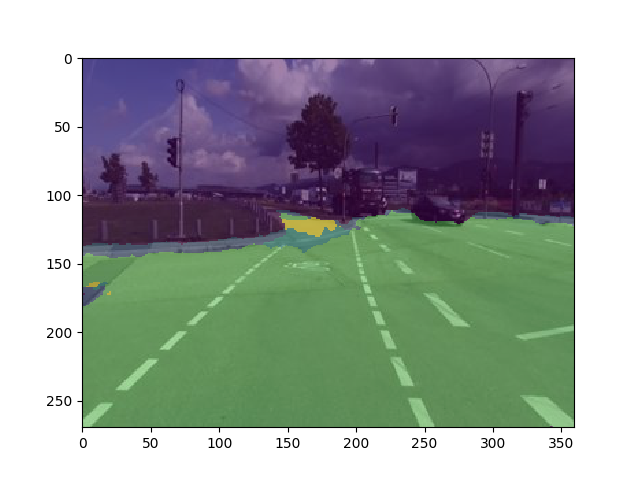
\includegraphics[width=\linewidth]{figures/experiments/results-obelix/1.png}
		\caption[Obelix Segmentation Result 1]{}
		\label{fig:obresult-1}
	\end{subfigure}
	\hfill
	\begin{subfigure}{.45\textwidth}
		\centering
		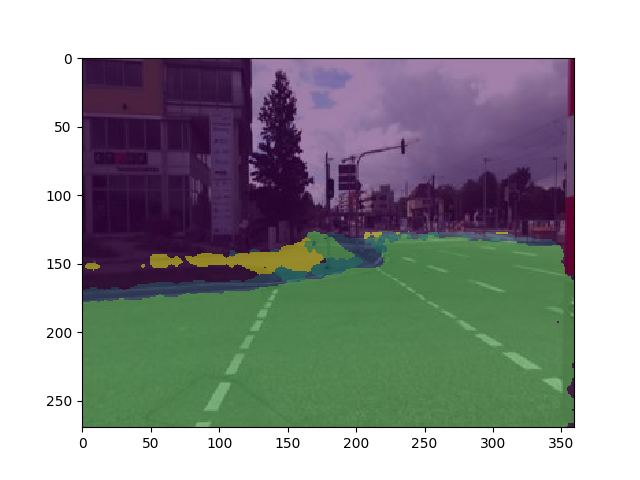
\includegraphics[width=\linewidth]{figures/experiments/results-obelix/2.png}
		\caption[Obelix Segmentation Result 2]{}
		\label{fig:obresult-2}
	\end{subfigure}
	
	\vspace{12pt}%------------
	
	\begin{subfigure}{.45\textwidth}
		\centering
		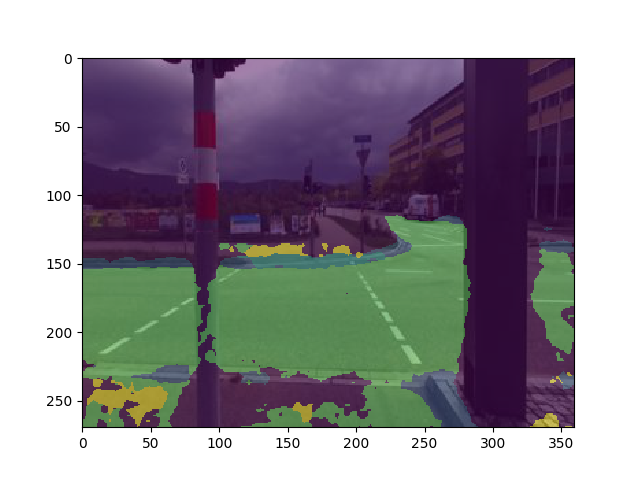
\includegraphics[width=\linewidth]{figures/experiments/results-obelix/3.png}
		\caption[Obelix Segmentation Result 3]{}
		\label{fig:obresult-3}
	\end{subfigure}
	\hfill
	\begin{subfigure}{.45\textwidth}
		\centering
		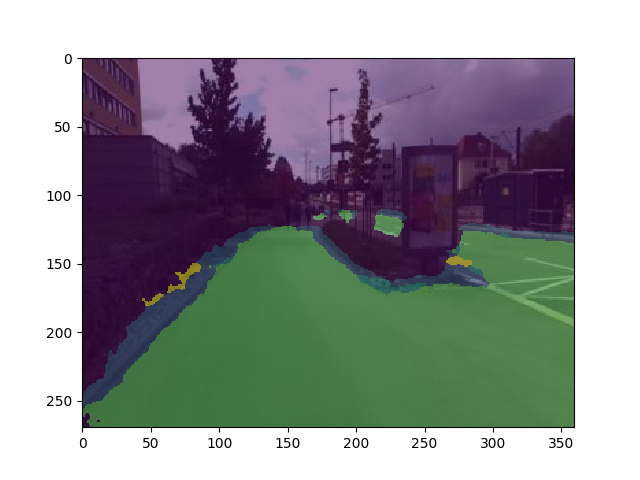
\includegraphics[width=\linewidth]{figures/experiments/results-obelix/4.png}
		\caption[Obelix Segmentation Result 4]{}
		\label{fig:obresult-4}
	\end{subfigure}

	\vspace{12pt}%------------
	
	\begin{subfigure}{.45\textwidth}
		\centering
		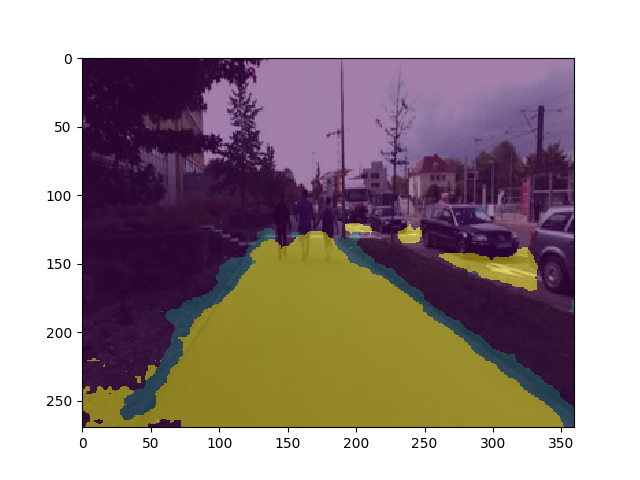
\includegraphics[width=\linewidth]{figures/experiments/results-obelix/5.png}
		\caption[Obelix Segmentation Result 5]{}
		\label{fig:obresult-5}
	\end{subfigure}
	\hfill
	\begin{subfigure}{.45\textwidth}
		\centering
		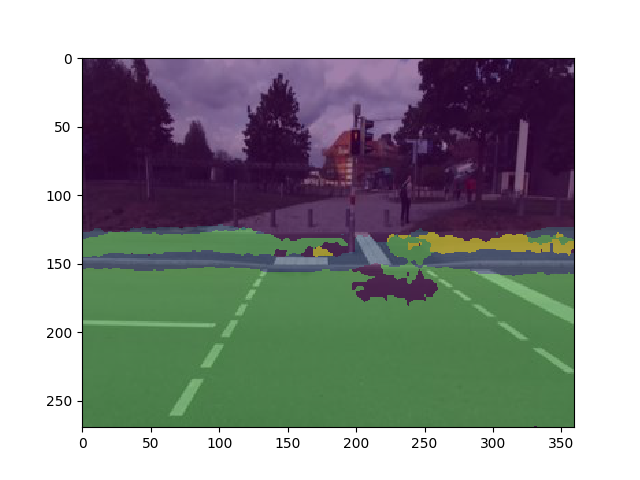
\includegraphics[width=\linewidth]{figures/experiments/results-obelix/6.png}
		\caption[Obelix Segmentation Result 6]{}
		\label{fig:obresult-6}
	\end{subfigure}

	\caption[Obelix Segmentation Results]{A sample of some segmentation results from the trained CurbNet model. The images are from the Obelix dataset. Green is road, yellow is sidewalk, blue is curb, turquoise is curb cuts, and purple is the ignore class. Figures \ref{fig:obresult-1} and \ref{fig:obresult-2} shows how the model is able to identify all of the different traversibility classes in the Obelix dataset even though it was only trained on the Mapillary dataset. Figure \ref{fig:obresult-3} shows curb cuts are sometimes also identified properly, as seen in the identification of the curb cut across the street, but not always, as seen in the curb cut directly in front of Obelix. Figures \ref{fig:obresult-4} and \ref{fig:obresult-5} shows a case where the network seems to be unable to decide if the sidewalk is a sidewalk or a road. In both cases, the sidewalk edge is marked as a curb, when it should not. Figure \ref{fig:obresult-6} shows a case where the left half of the sidewalk is labeled as road while the right half is labeled as sidewalk.}
	\label{fig:experiments-resultsobelix}
\end{figure}